% Comandos de dados - titulo do documento
\newcommand{\titulo}[1]{\title{#1}}
\newcommand{\imprimirtitulo}{\thetitle}

% Comandos de dados - autor (use \and para multiplos autores)
\newcommand{\autor}[1]{\author{#1}}
\newcommand{\imprimirautor}{\theauthor}

% Comandos de dados - data
\let\olddate\date
\renewcommand{\date}[1]{\AtBeginDocument{\olddate{#1}}}
\newcommand{\data}[1]{\date{#1}}
\newcommand{\imprimirdata}{
  \center
  S\~ao Leopoldo
  \thedate
}

% Comandos de dados - instituicao
\providecommand{\imprimirinstituicao}{}
\newcommand{\instituicao}[1]{\renewcommand{\imprimirinstituicao}{#1}}

% Comandos de dados - local
\providecommand{\imprimirlocal}{}
\newcommand{\local}[1]{\renewcommand{\imprimirlocal}{#1}}

% Comandos de dados - preambulo
\providecommand{\imprimirpreambulo}{}
\newcommand{\preambulo}[1]{\renewcommand{\imprimirpreambulo}{#1}}

% Comandos de dados - orientador
\providecommand{\imprimirorientadorRotulo}{}
\providecommand{\imprimirorientador}{}
\newcommand{\orientador}[2][\orientadorname]%
  {\renewcommand{\imprimirorientadorRotulo}{#1}%
   \renewcommand{\imprimirorientador}{#2}}

% Comandos de dados - coorientador
\providecommand{\imprimircoorientadorRotulo}{}
\providecommand{\imprimircoorientador}{}
\newcommand{\coorientador}[2][\coorientadorname]%
  {\renewcommand{\imprimircoorientadorRotulo}{#1}%
   \renewcommand{\imprimircoorientador}{#2}}

% Comandos de dados - tipo de trabalho
\providecommand{\imprimirtipotrabalho}{}
\newcommand{\tipotrabalho}[1]{\renewcommand{\imprimirtipotrabalho}{#1}}


\newcommand{\imprimircapa}{%
  \begin{capa}%
    \center
    \imprimirinstituicao
    \vfill
    \large\imprimirautor

    \vfill
    \begin{center}
      \MakeUppercase{\imprimirtitulo}
    \end{center}
    \vfill

    \large\imprimirlocal

    \large\imprimirdata

    \vspace*{1cm}
  \end{capa}
}

\newenvironment{capa}{\begin{titlingpage}}{\end{titlingpage}\cleardoublepage}

% ---
% Folha de rosto
%   usar \imprimirfolhaderosto* casodeseje imprimir algo no verso da
%   página no caso de estar no modo twoside. Util para imprimir a Ficha
%   Bibliografica. Porem, se estiver no modo oneside, a versao sem estrela
%   é identica.
\newenvironment{folhaderosto}[1][\folhaderostoname]{\clearpage}{\cleardoublepage}
\newenvironment{folhaderosto*}[1][\folhaderostoname]{\clearpage}{\newpage}%

% ---
% Conteudo padrao da Folha de Rosto
\makeatletter
\newcommand{\folhaderostocontent}{
  \begin{center}
    \imprimirinstituicao\vspace*{\fill}

    \large\imprimirautor

    \vspace*{\fill}\vspace*{\fill}
    \begin{center}
      \MakeUppercase{\imprimirtitulo}
    \end{center}
    \vspace*{\fill}

    \hspace{.45\textwidth}
    \begin{minipage}{.5\textwidth}
    	\singlespacing
       \imprimirpreambulo
     \end{minipage}
     \vspace*{\fill}

    \large\imprimirorientadorRotulo
    \imprimirorientador\par
    \vspace*{\fill}

    \large\imprimirlocal
    \par
    \large\imprimirdata
    \vspace*{1cm}

  \end{center}
}
\makeatother

\newcommand{\imprimirfolhaderostostar}[1]{%
  \begin{folhaderosto*}{#1}
     \folhaderostocontent
  \end{folhaderosto*}}

\newcommand{\imprimirfolhaderostonostar}[1]{%
  \begin{folhaderosto}{#1}
     \folhaderostocontent
  \end{folhaderosto}}

\makeatletter
\newcommand{\imprimirfolhaderosto}[1][\folhaderostoname]{%
   \@ifstar
     \imprimirfolhaderostostar
     \imprimirfolhaderostonostar
}
\makeatother


\documentclass[12pt]{article}
\usepackage{titling}
\usepackage{sbc-template}
\usepackage{graphicx,url}

\usepackage[brazil]{babel}   
\usepackage[utf8]{inputenc}  

\usepackage{multicol}
\usepackage{multirow}
\usepackage{setspace,lipsum}

\sloppy

\date{\today}

\title{
    Uma Apresentação do Modelo de Artigos da Sociedade Brasileira de Computação Adaptado pela Unisinos
}

\author{Roger D. Vieira\inst{1}}

\preambulo{Modelo canônico de Relatório Técnico e/ou Científico em conformidade
com as normas ABNT/SBC apresentado à comunidade de usuários \LaTeX.}

\address{Universidade do Vale do Rio dos Sinos (UNISINOS)\\
  Av. Unisinos, 950, Bairro Cristo Rei, São Leopoldo, RS -- Brasil
}

\instituicao{
    UNIVERSIDADE DO VALE DO RIO DOS SINOS - UNISINOS
    
    UNIDADE ACADÊMICA DE EDUCAÇÃO CONTINUADA
    
    ESPECIALIZAÇÃO EM BIG DATA, DATA SCIENCE E DATA ANALYTICS
}

\begin{document} 

\imprimircapa
\imprimirfolhaderosto

\maketitle

\begin{abstract}

This meta-paper describes the style to be used in articles and short papers according by SBC standards adapted to Unisinos necessities. Author should pay attention to limit of 10 lines in abstract and resumo. In both cases, they must be in the first page of the paper.
\end{abstract}
     
\begin{resumo} 
  Este meta-artigo descreve o estilo a ser usado na confecção de artigos e resumos de artigos em conformidade com as normas da SBC adaptadas às necessidades da Unisinos. O autor deve tomar cuidado para que o resumo (e o abstract) não ultrapassem 10 linhas cada, sendo que ambos devem estar na primeira
  página do artigo.
\end{resumo}


\section{Informações Gerais}


Todos os artigos e pôsteres (artigos curtos) submetidos para conferência da SBC, incluindo quaisquer documentos auxiliares, devem ser escritos em Ingês ou Português. O formato do artigo deverá ser A4 com uma única coluna, 3,5cm para margem superior,  2,5cm para a inferior e 3,5 para as margens laterais, sem cabeçalhos ou rodapés. A fonte principal deverá ser Time, tamanho nominal de 12 pontos, com 6 pontos de espaçamento entre cada parágrafo. Os números de páginas deverão ser suprimidos.

Artigos completos devem respeitar o limite de páginas definido por cada conferência. Conferências que publicam apenas resumos (abstracts) solicitam textos de \textbf{uma} página.

\section{Primeira Página} \label{sec:firstpage}

A primeira página deverá mostrar o título do artigo, os nomes e endereços dos autores, o \emph{abstract} em Inglês e o resumo em Português (resumos são necessários somente para artigos escritos em Português). O título deverá ser centralizado em toda a página, com fonte em negrito e 16 pontos de tamanho e 12 pontos de espaço anterior. Os nomes dos autores devem ser centralizados, com 12 pontos de tamanho de fonte, em negrito, todos dispostos na mesma linha, separados por vírgulas e com 12 pontos de distância após o título. 

Endereços devem ser centralizados, com fonte de 12 pontos, também com 12 pontos de espaçamento após o nome dos autores. Endereços de e-mail devem ser escritos usando-se a fonte Courier New, com tamanho nominal de 10 pontos, com 6 pontos de espaço antes e depois.

O \emph{abstract} e o resumo (caso necessário) devem ser escritos com fonte do tipo Times de 12 pontos, recuados em 0,8cm em ambos os lados. As palavras \emph{\textbf{Abstract}} e \textbf{Resumo} devem ser escritas em negrito e precedentes ao texto.

\section{CD-ROMs e Procedimentos Impressos}

Em algumas conferências, os artigos são publicados em CD-ROM enquanto somente o \emph{\textbf{abstract}} é publicado em procedimentos impressos. Neste caso, é solicitado que os autores preparem duas versões finais do artigo. Uma completa, para ser publicada no CD-ROM e outra contendo somente a primeira página, com o \emph{abstract} e o resumo (para artigos em Português).


\section{Seções e Parágrafos}

Os títulos das seções devem ser em negrito, tamanho de 13 pontos, alinhados à esquerda. Deve haver um espaço extra de 12 pontos antes de cada título. A numeração das seções é opcional. O primeiro parágrafo de cada senão não deverá ter recuo, enquanto as primeiras linhas dos parágrafos subsequentes devem ser recuadas em 1,27cm. 


\subsection{Subseções}

Os títulos de subseções devem estar em negrito, com tamanho de 12 pontos e alinhados à esquerda.

\section{Figuras e Legendas}\label{sec:figs}

As legendas de figuras e tabelas devem ser centralizadas se menores que uma linha (Figura~\ref{fig:exampleFig1}), caso contrário, deverão ser justificadas e recuadas em 0,8cm em ambas as margens, como mostrado na Figura~\ref{fig:exampleFig2}. A fonte das legendas deverá ser Helvetica, de tamanho 10, em negrito, com 6 pontos de espaços antes e depois de cada legenda.

\begin{figure}[ht]
\centering
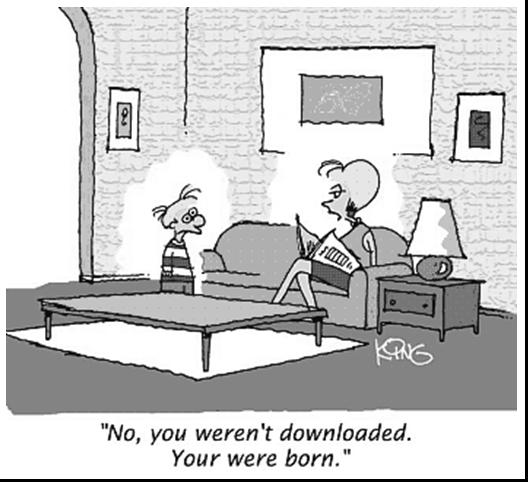
\includegraphics[width=.5\textwidth]{fig1.jpg}
\caption{Uma figura típica}
\label{fig:exampleFig1}
\end{figure}

\begin{figure}[ht]
\centering
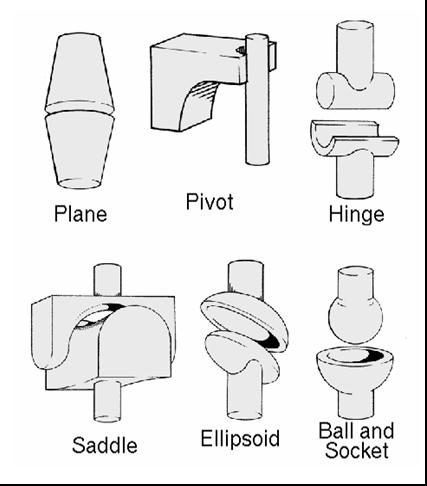
\includegraphics[width=.3\textwidth]{fig2.jpg}
\caption{Este é um exemplo de legenda de figura que ocupa mais de uma linha, cuja justificação deverá considerar as margens mencionadas na Seção~\ref{sec:figs}.}
\label{fig:exampleFig2}
\end{figure}

Em tabelas, tente evitar o uso de fundos coloridos ou sombreados, além de linhas de moldura grossas, duplas ou desnecessárias. Quando apresentar dados empíricos, não use mais casas decimais do que as garantidas pelas suas precisões e reprodutibilidades. Legendas de tabelas devem ser colocadas antes da tabela (veja Tabela~\ref{tab:exTable1}) e a fonte deverá ser também Helvetica, 10 pontos, em negrito, com 6 pontos de espaço antes e depois de cada legenda.


\begin{table}[ht]
\centering
\caption{Variáveis a serem consideradas na avalição das técnicas de interação.}
\label{tab:exTable1}
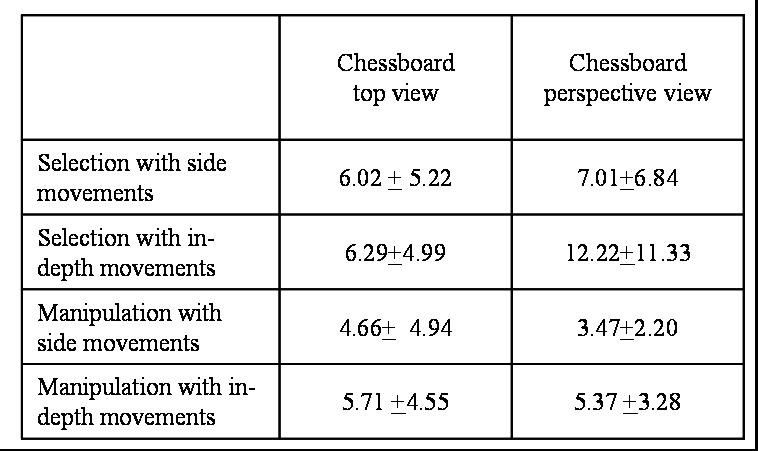
\includegraphics[width=.7\textwidth]{table.jpg}
\end{table}

\section{Imagens}

Todas as imagens e ilustrações devem ser em preto-e-branco ou tons de cinza, excetuando-se aquelas que serão disponívels eletronicamente (em CD-ROMs, internet, etc...). A resolução da imagem no artigo será de 600dpi para imagens em preto-e-branco e 150-300dpi para imagens em tons de cinza. Não incluir imagens com resoluções excessivas, já que elas podem levar horas para serem impressas, sem alguma diferença visível no resultado.

\section{Referências}

As referências bibliográficas devem ser únicas e uniformes. Recomendamos que as referências aos nomes dos autores estejam entre chaves, ex.: \cite{knuth:84}.

As referências devem ser listadas usando fonte de 12 pontos, com 6 pontos de espaço entre cada uma. A primeira linha de cada referência não deve ser recuada, enquanto as linhas subsequentes devem possuir recuo de 0,5cm.

\bibliographystyle{sbc}
\bibliography{sbc-template}

\end{document}
